\documentclass[letterpaper]{article} % DO NOT CHANGE THIS
\usepackage[submission]{aaai2027}  % DO NOT CHANGE THIS
% The serif, sans-serif, and monospaced fonts are loaded automatically by
% aaai2027.sty (newtxtext, helvet, courier). DO NOT add \usepackage{times},
% \usepackage{helvet}, \usepackage{courier}, or any other font package.
\usepackage[hyphens]{url}  % DO NOT CHANGE THIS
\usepackage{graphicx} % DO NOT CHANGE THIS
\urlstyle{rm} % DO NOT CHANGE THIS
\def\UrlFont{\rm}  % DO NOT CHANGE THIS
\usepackage{natbib}  % DO NOT CHANGE THIS AND DO NOT ADD ANY OPTIONS TO IT
\usepackage{caption} % DO NOT CHANGE THIS AND DO NOT ADD ANY OPTIONS TO IT
\frenchspacing  % DO NOT CHANGE THIS

% Recommended to typeset algorithms.
\usepackage{algorithm}
\usepackage{algorithmic}

% Recommended to typeset listings.
\usepackage{newfloat}
\usepackage{listings}
\usepackage{amsmath}
\usepackage{amssymb}
\DeclareCaptionStyle{ruled}{labelfont=normalfont,labelsep=colon,strut=off} % DO NOT CHANGE THIS
\lstset{%
    basicstyle={\footnotesize\ttfamily},
    numbers=left,numberstyle=\footnotesize,xleftmargin=2em,
    aboveskip=0pt,belowskip=0pt,
    showstringspaces=false,tabsize=2,breaklines=true}
\floatstyle{ruled}
\newfloat{listing}{tb}{lst}{}
\floatname{listing}{Listing}

% Recommended for better-looking tables.
\usepackage{booktabs}

\pdfinfo{
/TemplateVersion (2027.1)
}

\setcounter{secnumdepth}{0} % May be changed to 1 or 2 if section numbers are desired.

% Title must be in mixed case.
\title{WACBench: Evaluating Strategic Adaptation in LLM Agents through Executable Policies}

\author{Anonymous Submission}
\affiliations{}

\begin{document}

\maketitle

% Large language models are increasingly moving from assistant-style interaction toward roles that may require consequential, repeated decision making.

\begin{abstract}
Large language models (LLMs) are increasingly considered not only as assistants but as agents that may formulate and execute consequential strategies. Yet existing benchmarks often emphasize isolated actions or task completion, leaving unclear whether models can construct persistent policies and revise them under scarcity, uncertainty, delayed consequences, and strategic interdependence. We introduce WACBench, a code-mediated multi-agent benchmark built on a repeated resource-allocation game. In each meta-round, agents submit executable bidding policies that govern a complete episode and can be frozen, replayed, and inspected. Treating executable policy as the unit of evaluation removes repeated policy-to-action translation and enables comparison of stated rationale, implemented decision rules, and realized trajectories. We compare a shared self-policy-and-outcome feedback protocol with a condition that additionally reveals opponents' previous policies. Across multiple LLM backends, both feedback conditions improve initial revisions, while opponent-policy access sustains later gains in role-balanced survival and induces behavioral and structural convergence. WACBench provides a reproducible framework for evaluating policy construction and adaptation and reveals how access to strategic information reshapes policy revision.
\end{abstract}
% TODO: Add the anonymized code URL before submission.
% \noindent\textbf{Code} --- \url{https://anonymous-code-host.example/WACBench}


% Uncomment the following to link to code, datasets, or an extended version.
% Keep this block between the abstract and the main body, and avoid de-anonymizing links.
\begin{links}
    \link{Code}{https://anonymous.4open.science/your-repository}
%     \link{Datasets}{https://anonymous.4open.science/your-dataset}
%     \link{Extended version}{https://anonymous.4open.science/your-extended-version}
\end{links}

\section{Introduction}

Large language models (LLMs) are increasingly considered not only as
assistants that recommend actions, but also as agents that may formulate and
execute strategies on behalf of users. In resource allocation, bidding,
procurement, and organizational planning, decisions repeat, consequences may
be delayed, and success depends on both an uncertain environment and other
decision makers. Evaluating such agents therefore requires more than isolated
responses or task completion: it requires testing whether a model can
construct a persistent decision rule, execute it reliably, and improve it
through experience.

Existing agent benchmarks have substantially advanced the evaluation of
multi-step reasoning, tool use, open-ended task completion, and social
interaction~\cite{liu2023agentbench,mialon2023gaia,zhou2024sotopia,zhu2025multiagentbench}.
Classical games complement them with explicit objectives and controlled tests
of particular strategic phenomena, including rational action selection,
strategic reasoning, and budget management
~\cite{fan2024rational,duan2024gtbench,huang2025gamabench,chen2023aucarena}.
As LLM agents improve, evaluation can ask whether these abilities compose
across long horizons, stochastic dynamics, asymmetric constraints, and
multiple competitors. The Water
Allocation Challenge (WAC) provides this stress test while retaining explicit
rules and objectively measurable outcomes~\cite{mao2025alympics}.

These environments reveal important aspects of decision making, but their
primary evaluation unit is often an interaction-step action. The observed
trajectory then combines at least three factors: the quality of the intended
strategy, its repeated translation into actions, and changes in the
surrounding policy population. This makes it difficult to determine whether
success reflects a stable state-dependent rule or a sequence of locally
generated responses. Prior work also shows that a refined belief can be
overlooked or modified during action selection~\cite{fan2024rational},
demonstrating a potential discontinuity between strategic reasoning and
execution.

Contemporary LLM code-generation capabilities make it practical to represent
a strategy as an executable decision rule rather than only a rationale or
action sequence. WACBench therefore treats an \emph{executable policy} as the
unit of decision making. An LLM submits a strategy rationale and a Python
policy mapping observable states to bids; the simulator invokes the same code
throughout the episode. The implemented rule is thus persistent, every action
is traceable, and the rationale, policy, and trajectory can be compared and
replayed. Program-based strategies have supported analysis of code-conditioned
behavior in open-source games~\cite{sistla2025opensourcegames}; WACBench uses
this auditability to evaluate policy construction and revision.
Code mediation removes potential reasoning--action translation error while
preserving rationale--policy disagreement as an observable diagnostic.
Because submitted policies can be frozen and recombined without further LLM
calls, WACBench also supports counterfactual comparisons unavailable from a
single realized action sequence.

We introduce \textbf{WACBench}, a code-mediated multi-agent benchmark built
on WAC. Five agents compete for limited daily water over a 20-day episode.
In each meta-round, an LLM generates a policy for a complete episode and may
revise it only before the next meta-round. We operationalize strategic
adaptation as constructing an effective persistent policy, improving it after
feedback, and sustaining improvement across repeated revisions. Long-horizon
planning, state-dependent risk management, and competition are demands
jointly imposed by the environment rather than independent scoreboards.

The benchmark couples simulator-grounded outcomes with policy-level controls.
Role-balanced multi-seed replay measures performance across asymmetric
assignments and supply sequences. Frozen-opponent counterfactuals determine
whether a focal revision improves against unchanged competitors, while a
fixed non-LLM policy calibrates the scale of tournament outcomes. Controlled
behavioral and structural probes characterize how policy populations change,
and evidence-grounded failure analysis explains recurrent breakdowns. These
components separate overall policy quality, effective unilateral revision,
and population-level co-adaptation.

We demonstrate this framework by studying whether opponents' previous
decision rules provide a reusable signal for revision. Both conditions reveal
an agent's own previous policy and all agents' survival durations. Under
\textbf{Outcome Feedback (OF)}, opponent policies remain hidden;
\textbf{Outcome-and-Policy Feedback (OPF)} additionally reveals their
preceding-round programs. Frozen-opponent replays confirm effective initial
revision under both protocols. Across three meta-rounds, OF then plateaus
whereas OPF sustains role-balanced survival gains, moves beyond the fixed
reference, and induces behavioral and structural convergence. Thus, OF/OPF
serves as a controlled demonstration of the policy-level questions WACBench
is designed to answer.

Our contributions are summarized as follows:

\begin{itemize}
    \item We introduce WACBench, a code-mediated benchmark that evaluates
    strategic LLM agents through persistent executable policies in a
    repeated, asymmetric, and resource-constrained environment.
    
    \item We provide a policy-level evaluation protocol combining
    role-balanced multi-seed replay, frozen-opponent counterfactuals, and a
    fixed non-LLM reference to distinguish policy quality, effective
    revision, and co-adaptation.
    
    \item Using opponent-policy access as an information intervention, we
    show sustained later-round survival gains together with behavioral and
    structural policy convergence.
\end{itemize}
\section{Related Work}

\paragraph{LLM agent evaluation.}
General agent benchmarks emphasize multi-step task completion, tool use,
and interaction, while multi-agent benchmarks additionally study social
coordination and competition~\cite{liu2023agentbench,mialon2023gaia,zhou2024sotopia,zhu2025multiagentbench}.
WACBench instead evaluates a policy that is generated once and then acts
without further LLM intervention throughout an episode. This separates
policy construction from repeated execution and permits exact replay and
behavioral probing.

\paragraph{LLMs in games and auctions.}
Prior work uses classical games and auction environments to examine
rational choice, strategic reasoning, and budget management
~\cite{fan2024rational,duan2024gtbench,huang2025gamabench,chen2023aucarena}.
WACBench complements these controlled tests by composing long horizons,
stochastic scarcity, asymmetry, and multi-agent competition.
Recent work also evaluates a single CFO-style agent over a long-horizon,
partially observable enterprise resource-allocation simulation
~\cite{han2026enterprisearena}. WACBench studies persistent-policy revision
among simultaneous competitors, with common-seed and frozen-opponent replays.
Alympics introduced WAC as a pilot environment for empirical game-theoretic
analysis and combined objective game records with human ratings of broad
strategic abilities~\cite{mao2025alympics}. We retain WAC's scarcity,
asymmetry, and survival dynamics, but shift the unit of evaluation from a
natural-language action sequence to controlled revision of executable
policies.

\paragraph{Program-mediated strategies.}
Program-based games make strategies reproducible and inspectable, and have
been used to study code-conditioned cooperation and exploitation
~\cite{sistla2025opensourcegames}. WACBench uses the same auditability for a
different purpose. Rather than allowing a program to inspect an opponent's
source during play, OPF reveals only the opponents' preceding-round programs
before the next policy is submitted. This links rationale, code, and realized
trajectory while making policy visibility a controlled cross-round
intervention.
\section{The Repeated Water Allocation Game}
The Water Allocation Challenge (WAC), originally introduced
as a pilot environment in Alympics~\cite{mao2025alympics},
is a repeated resource-allocation game in which multiple agents compete for
limited daily water while managing health, budget, and long-term survival.
WAC provides the strategic environment for WACBench by combining scarce
resources, asymmetric participants, uncertain future supply, and short- versus
long-term tradeoffs within a controlled simulation.

\subsection{Game Overview}

Each episode spans $T=20$ simulation days. At the beginning of an
episode, each agent is assigned a role specifying its daily salary $s_i$
and water requirement $w_i$. All roles begin with the same health,
budget, and no-water penalty state: $H_{i,1}=8$, $B_{i,1}=0$, and
$c_{i,1}=1$, with maximum health $H_{\max}=10$. The medium-scarcity
setting used in our experiments samples each day's integer supply as
$S_t\sim\operatorname{Unif}\{15,\ldots,25\}$. The current supply is
announced before all living agents submit simultaneous bids, but
current-day opponent bids remain hidden. The resulting four-stage daily loop
is summarized in the central panel of Figure~\ref{fig:wacbench_framework}.

\begin{table}[t]
    \centering
    \small
    \setlength{\tabcolsep}{9pt}
    \caption{Asymmetric WAC role profiles.}
    \label{tab:role-profiles}
    \begin{tabular}{lrr}
        \toprule
        Role & Water requirement $w_i$ & Daily salary $s_i$ \\
        \midrule
        Alex  & 13 & 70  \\
        Bob   & 9  & 90  \\
        Cindy & 13 & 150 \\
        David & 7  & 80  \\
        Eric  & 8  & 140 \\
        \bottomrule
    \end{tabular}
\end{table}

The names are inherited from WAC and serve only as role identifiers; they
imply no personas.
As Table~\ref{tab:role-profiles} shows, asymmetry refers to the joint
salary--requirement profiles rather than to different initial health
states. These profiles create different strategic constraints: high water
requirements make allocation more difficult when little supply remains,
while low salaries limit the bids that can be sustained over the episode.
The complete permutation evaluation rotates every model through every role
so that these structural advantages do not determine a model's aggregate
score.

Formally, let $i \in \{1,\ldots,N\}$ denote an agent and $t$ denote the
day. In addition to the fixed $s_i$ and $w_i$, each agent maintains budget
$B_{i,t}$, health $H_{i,t}$, and a no-water penalty counter $c_{i,t}$. The
counter determines the health penalty if the agent fails to obtain water
on the current day. Agents observe the announced supply and current public
states before choosing $b_{i,t}$, but do not observe other agents'
current-day bids.

\subsection{Daily Bidding, Allocation, and State Transitions}

At the start of each day, each living agent receives its
salary. Let
\begin{equation}
    \widetilde{B}_{i,t}=B_{i,t}+s_i
\end{equation}
denote the budget available for that day's auction.
The environment ranks positive feasible bids in descending order, with
ties first resolved in favor of the lower water requirement. Remaining
exact ties are resolved by a reproducible seeded tie-break. It then visits
the ranked list and allocates water to any agent whose requirement fits the
remaining supply, subtracting that requirement before considering the next
agent. Let $z_{i,t}\in\{0,1\}$ indicate whether agent $i$ receives water
on day $t$.

A winning agent pays its bid, while a non-winning agent pays
nothing:
\begin{equation}
    B_{i,t+1}
    =
    \widetilde{B}_{i,t}-z_{i,t}b_{i,t}.
\end{equation}

The no-water penalty counter is updated as
\begin{equation}
    c_{i,t+1}
    =
    \begin{cases}
        1, & z_{i,t}=1,\\
        c_{i,t}+1, & z_{i,t}=0.
    \end{cases}
\end{equation}

Health then evolves according to
\begin{equation}
    H_{i,t+1}
    =
    \begin{cases}
        \min(H_{\max},H_{i,t}+2), & z_{i,t}=1,\\
        H_{i,t}-c_{i,t}, & z_{i,t}=0.
    \end{cases}
\end{equation}
An agent is eliminated when its health reaches zero or below.

\subsection{Strategic Challenges}

WAC jointly tests long-horizon budget allocation, state-dependent risk
response, and competition under asymmetric roles: aggressive bids may secure
short-term survival but deplete later resources, while bid effectiveness
depends on both the agent's current risk and its opponents' policies.

\section{WACBench}

WACBench evaluates strategic LLM agents through policies rather than
independently generated daily actions. Each submitted policy remains the
agent's decision rule for a complete episode, after which it can be revised,
frozen for replay, or evaluated on controlled states.

\begin{figure*}[t]
    \centering
    \includegraphics[width=\textwidth]{framework_v5.pdf}
    \caption{Overview of WACBench. The central green panel summarizes the
    four-stage daily WAC loop: announce supply, collect simultaneous bids,
    allocate water, and update agent states. Submitted rationales, executable
    policies, traces, and outcomes are stored for condition-dependent
    meta-round feedback and post-hoc evaluation. Judge annotations are
    secondary and never affect gameplay or primary outcomes.}
    \label{fig:wacbench_framework}
\end{figure*}

\subsection{Benchmark Overview}

As shown in Figure~\ref{fig:wacbench_framework}, the experiment controller
assigns backends and roles, validates submitted policies, executes each
meta-round, and stores the resulting code, traces, and outcomes. Selected
artifacts construct OF or OPF feedback for the next revision; post-hoc
diagnostics read the store without affecting gameplay.

The benchmark separates three objects that action-level evaluation can
conflate: the model's stated rationale, its implemented policy, and the
trajectory produced when that policy is executed. Simulator-grounded survival
and adaptation are the primary evidence of decision quality. Code validity,
controlled policy probes, and judge annotations characterize reliability and
failure mechanisms without replacing realized outcomes.

\subsection{Code-Mediated Agent Policies}

In each meta-round, an LLM agent receives a profile, the current game setup,
and condition-dependent information about other agents. The agent produces
two artifacts: a concise natural-language strategy rationale and executable
Python policy code. Each policy implements
\texttt{get\_bid(day\_context, my\_status, opponents\_status)}, which the
environment calls on every simulation day to obtain one bid. The input
\texttt{day\_context} contains the current day and
announced supply; \texttt{my\_status} contains health, available budget, and
the no-water counter; and \texttt{opponents\_status} contains the public
current states and recent past-day observations of other agents. Current-day
opponent bids are never available when a policy acts.

Code mediation serves four evaluation purposes. First, it makes the policy
persistent: the simulator invokes the submitted decision rule rather than
asking the LLM to reconstruct a strategy each day. Second, it provides
policy--execution fidelity: every realized bid is attributable to a specific
program and observed state, subject to explicit validation and runtime checks.
Third, a frozen policy can be replayed under common supply sequences or probed
on controlled states. Fourth, the natural-language rationale, implemented
logic, and resulting trajectory can be audited separately. The design thus
removes repeated translation from policy to action, but deliberately retains
rationale--policy disagreement as a detectable failure mode.

\subsection{Meta-Round Adaptation and Feedback Conditions}
A meta-round is one policy-revision cycle. At the
beginning of meta-round $k$, each agent generates one policy
$\pi_i^{(k)}$; the simulator executes one $T$-day episode with
that policy fixed throughout; and selected artifacts construct
feedback for meta-round $k+1$. Policies may be revised only
between meta-rounds. We use $k\in\{1,\ldots,K\}$ for
meta-rounds and reserve $t\in\{1,\ldots,T\}$ for days.

For $k>1$, both feedback conditions provide the agent's own
previous policy and all previous survival durations. Here
$D_j^{(k-1)}\in\{1,\ldots,T\}$ is the number of days agent $j$
survived in meta-round $k-1$, with $T$ denoting episode
completion. We denote this common revision memory by
\begin{equation}
    M_i^{(k)}
    =
    \left\{\pi_i^{(k-1)},
    D_1^{(k-1)},\ldots,D_N^{(k-1)}\right\}.
\end{equation}
Under \textbf{Outcome Feedback (OF)}, $F_{i,\mathrm{OF}}^{(k)}=M_i^{(k)}$.
No opponents' previous policies, bids, allocation records, daily
trajectories, or intermediate state histories are revealed.

Under \textbf{Outcome-and-Policy Feedback (OPF)}, the agent
receives the common revision memory together with the strategy
code submitted by every opponent in the previous meta-round:
\begin{equation}
    F_{i,\mathrm{OPF}}^{(k)}
    =
    M_i^{(k)}
    \cup
    \{\pi_j^{(k-1)}:j\neq i\}.
\end{equation}

The two conditions share the simulator, role assignments, own-policy memory,
outcome feedback, and within-episode observation interface. Their comparison
estimates the effect of adding opponents' policy representations within this
fixed feedback protocol. Meta-round one has no previous-round memory and
serves as a pre-feedback baseline within each condition. Because OF and OPF
use separate policy-generation runs, their MR1 policies need not be identical;
we therefore estimate policy-access effects as matched differences in changes
from the respective MR1 baselines.

\subsection{Memory, Trace Storage, and Policy Evaluation}

After each episode, WACBench stores the rationale, executable policy, daily
traces, and final outcome. Condition-allowed artifacts form subsequent
feedback, while the complete record supports deterministic outcome metrics
and post-hoc diagnosis. Judges read this evidence only after execution and
never affect gameplay.

\subsection{Evidence-Grounded Failure Analysis}

WACBench analyzes the stored rationale, executable policy, and active-day
trajectory for each death in the original policy-generation episodes. Death,
affordable threshold misses, actual payments, and prior overpayment are
reconstructed from simulator records. Same-day opponent bids and winning
thresholds are used only as ex-post diagnostic evidence.

The diagnostic first distinguishes whether the policy is the dominant cause,
whether policy and adverse context jointly contribute, whether no clear
policy failure is supported, or whether evidence is insufficient. For the
first two cases, a judge assigns one primary mechanism and up to two
contributing mechanisms. The headline analysis uses only the primary
mechanism; contributing labels are retained in the released annotations.
We report four policy mechanisms:
\begin{itemize}
    \item \textbf{Fatal undercommitment:} a reserve, cap, or fixed target
    keeps an affordable critical bid too low.
    \item \textbf{Winner's-curse overpayment:} premiums paid on early wins
    consume funds needed for later survival.
    \item \textbf{Emergency-response failure:} the risk-to-bid mapping
    escalates too late, in the wrong direction, or is overridden in a lethal
    state.
    \item \textbf{Competitive-threshold miscalibration:} the opponent-price
    estimator targets the wrong bid range.
\end{itemize}

We separately compute \emph{disadvantaged-role exposure}: whether a death
occurs in a role whose salary is below the within-game median and whose water
requirement is above the median. This deterministic flag identifies adverse
initial resources rather than a policy error or a causal explanation of
death. Other contextual contributors include unaffordable competition,
scarcity, and opponent-bid outliers. A rare allocation-context label is
retained in the released annotations but not used as a headline mechanism.

Two independently queried LLM judges (temperature zero) receive the same
structured evidence with the acting model's identity hidden. For each
displayed mechanism, a death receives score 1 if both judges select it as
primary, 0.5 if one selects it, and 0 otherwise. The displayed percentages
use all deaths for that model as the denominator. The disadvantaged-role
column may overlap with the primary mechanism, while omitted no-primary and
rare allocation-context diagnoses mean that the four policy columns need not
sum to 100\%. The judges diagnose failed trajectories after execution;
simulator-grounded WACScore and mortality remain the primary outcomes.

\section{Experimental Setup}

\subsection{Models, Conditions, and Replays}

We evaluate Claude Sonnet 5, DeepSeek V4 Flash, Gemini 3.5 Flash,
GPT-5.4, and GPT-5.4 Nano. The evaluation enumerates all $5!=120$
one-to-one permutations of these five models across the five asymmetric
roles, so every model appears equally often in every role. Let
$\mathcal{A}$ denote this set of permutations, and let
$a\in\mathcal{A}$ denote one such permutation. Each permutation is run for
three meta-rounds under OF and OPF.

Policy generation and revision use one shared supply sequence, so each model
revises from the same realized experience. We then freeze every submitted
policy and replay the MR1--MR3 policy sets on the experienced sequence and
four held-out supply sequences. Replays assess whether a revision transfers
beyond the trajectory that produced its feedback and provide no further
opportunities for revision. Exact seed identifiers are reported in the
appendix.

\subsection{Metrics and Statistical Analysis}

Our primary outcomes are WACScore and mortality. Let $T$ be the episode
horizon, $\mathcal{R}$ the roles, $\mathcal{E}_{m,r}$ the evaluation episodes
in which model $m$ occupies role $r$, and $D_{m,r,e}$ its survival duration.
We define
\begin{equation}
    \operatorname{WACScore}(m)
    =
    \frac{100}{|\mathcal{R}|T}
    \sum_{r\in\mathcal{R}}
    \frac{1}{|\mathcal{E}_{m,r}|}
    \sum_{e\in\mathcal{E}_{m,r}}D_{m,r,e}.
\end{equation}
WACScore is the role-balanced percentage of the episode survived. Mortality
is the corresponding role-balanced percentage of episodes in which a policy
dies before the horizon. Higher WACScore and lower mortality are better.
Because both outcomes arise from strategic competition, they are
population-conditioned measures rather than context-free model scores: every
comparison fixes the opponent-policy pool, role permutations, and supply
sequences.

Cross-meta-round changes measure adaptation. Because OF and OPF have separate
MR1 realizations, the policy-access contrast is estimated as the matched
difference between their changes from the respective MR1 baselines; raw
condition levels are descriptive. We first average replay seeds within each
experiment and then bootstrap the 120 matched experiment clusters, keeping
the five strategically coupled agents, both conditions, and all meta-rounds
together.

To test whether a revision helps independently of simultaneous changes by
other agents, Frozen-Opponent Survival Gain (FOSG) replaces only focal policy
$\pi_i^{(1)}$ with its MR2 revision while retaining all MR1 opponent policies:
\begin{equation}
    \mathrm{FOSG}
    =
    \mathbb{E}_{a,i,s}\!\left[
        D_i\!\left(\pi_i^{(2)},\pi_{-i}^{(1)};s\right)
        -
        D_i\!\left(\pi_i^{(1)},\pi_{-i}^{(1)};s\right)
    \right],
\end{equation}
where $a$ indexes the 120 permutations described above, $i$ is the focal
agent, $s$ indexes replay supply sequences, and $D_i$ is the focal agent's
survival duration. Positive FOSG indicates an effective focal revision against
unchanged opponents. Its OF--OPF contrast tests whether policy access improves
the first revision.

To characterize collective policy dynamics, we evaluate each submitted
policy on the same grid of 144 controlled states. Behavioral Policy Distance
(BPD) is the within-experiment mean pairwise RMSE between feasible bids after
normalization by available budget; lower BPD means that policies respond more
similarly to the same states. A normalized-AST analysis provides a structural
robustness check. Supplementary analyses further probe counterfactual
planning, risk response, and structural similarity.

\subsection{Non-LLM Reference Policy}

We calibrate policy quality with one fixed, interpretable risk-aware pacing
heuristic. On day $t$, it computes a sustainable bid
$p_t=[\widetilde{B}_{i,t}+(T-t)s_i]/(T-t+1)$ from the budget available after
the current salary payment and the role's known future salary.
It bids $0.5p_t$ when safe, $p_t$ when two consecutive losses would be fatal,
and $2p_t$ when the current loss would be fatal. In the latter two states, it
also bids at least one unit above the median positive previous-day bid of
living opponents. All constants are fixed without search. The policy observes
no future supply or current-day opponent bids and never receives feedback or
revises.

For every condition, assignment, meta-round, focal role, and replay seed, we
replace only the focal LLM policy with the role-parameterized heuristic while
holding the four opponent policy programs fixed. This yields 18,000 paired
replacements. Positive LLM-minus-reference WACScore differences favor the LLM;
negative mortality differences favor the LLM. Since the heuristic is fixed,
changes in its absolute outcomes across meta-rounds reflect changing opponent
policy pools rather than heuristic adaptation.

\section{Results}

\subsection{Policy Effectiveness and Benchmark Calibration}

Table~\ref{tab:outcome-performance} provides descriptive context for the
adaptation analysis by reporting simulator-grounded outcomes for revised
policies in MR2--MR3. The population-conditioned estimates reveal two broad
performance tiers: Gemini 3.5 Flash, Claude Sonnet 5, and GPT-5.4 form the
higher-performing group, followed by DeepSeek V4 Flash and GPT-5.4 Nano.
The reference row places the same fixed heuristic in the corresponding
opponent pools; baseline-adjusted policy-access effects are analyzed next.

\begin{table}[t]
    \centering
    \small
    \setlength{\tabcolsep}{3pt}
    \caption{Simulator-grounded performance over MR2--MR3 and five fixed
    supply sequences. LLM rows use submitted revised policies; the heuristic
    row uses the same fixed rule against the corresponding opponent pools.
    Estimates are role-balanced, Avg. is the unweighted condition mean, and
    backend names are abbreviated; full names appear in the Experimental
    Setup. Best point estimates in each column are bolded.}
    \label{tab:outcome-performance}
    \begin{tabular}{lrrr rrr}
        \toprule
        & \multicolumn{3}{c}{WACScore $\uparrow$}
        & \multicolumn{3}{c}{Mortality (\%) $\downarrow$} \\
        \cmidrule(lr){2-4}\cmidrule(lr){5-7}
        Model / policy & OF & OPF & Avg. & OF & OPF & Avg. \\
        \midrule
        Gemini 3.5 & \textbf{86.47} & \textbf{87.05} & \textbf{86.76}
                   & 25.75 & \textbf{25.08} & \textbf{25.42} \\
        Claude S5  & 86.17 & 84.05 & 85.11 & \textbf{25.00} & 28.67 & 26.83 \\
        GPT-5.4    & 84.27 & 81.72 & 83.00 & 27.58 & 31.08 & 29.33 \\
        DeepSeek V4 & 69.04 & 67.84 & 68.44 & 45.83 & 46.58 & 46.21 \\
        GPT-5.4 Nano & 50.95 & 65.35 & 58.15 & 66.42 & 48.83 & 57.62 \\
        \midrule
        Heuristic & 75.16 & 74.74 & 74.95 & 35.77 & 36.68 & 36.23 \\
        \bottomrule
    \end{tabular}
\end{table}

Paired replacement separates model policy quality from the raw tournament
outcomes. Across both protocols, Gemini, Claude, and GPT-5.4 outperform the
heuristic in WACScore and mortality, with all paired intervals excluding zero.
DeepSeek and GPT-5.4 Nano remain below the reference, while OPF substantially
narrows Nano's deficit. The fixed reference therefore distinguishes policies
that surpass a simple adaptive rule and anchors the practical scale of
tournament outcomes.

\subsection{From Effective Revision to Sustained Adaptation}

We first ask whether the initial revisions improve the focal policy rather
than merely benefiting from concurrent opponent changes. Across 6,000 paired
replays with all MR1 opponents frozen, replacing the focal MR1 policy by its
MR2 revision increases survival by 0.38 days under OF and 0.57 days under
OPF, with both intervals excluding zero. Both conditions therefore produce
effective first revisions; the longitudinal analysis below identifies where
their adaptation trajectories separate. Full FOSG intervals and model-level
estimates appear in the appendix.

We next replay each complete MR1--MR3 policy set under the same five supply
sequences. MR1 is the pre-feedback baseline, and policy-access effects use the
matched changes defined above. MR1--MR2 measures the first revision;
MR2--MR3 distinguishes continued improvement from saturation or regression.

\begin{figure}[t]
    \centering
    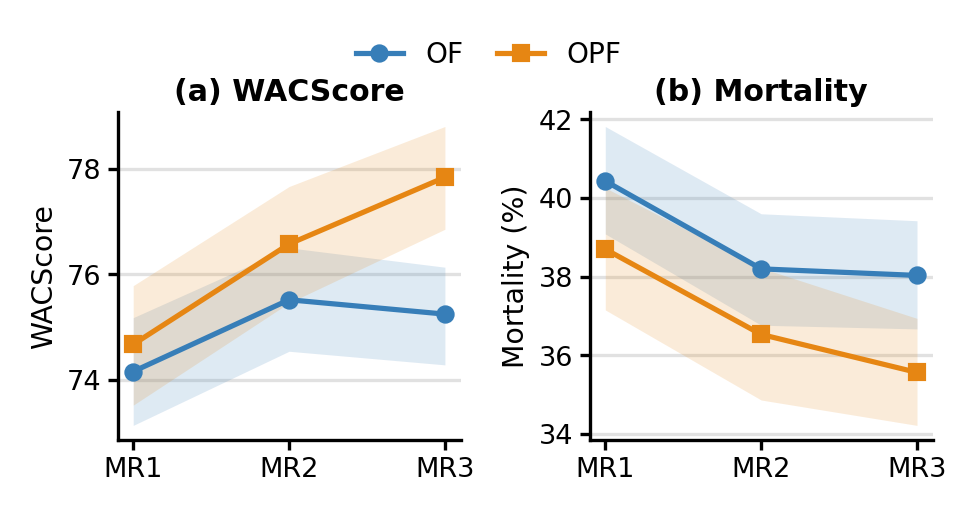
\includegraphics[width=\linewidth]{adaptation_trajectories.png}
    \caption{Cross-meta-round adaptation under Outcome Feedback (OF) and
    Outcome-and-Policy Feedback (OPF). Policies are replayed under five fixed
    supply sequences. Points are role-balanced estimates after averaging
    seeds within experiments; bands are 95\% matched experiment-cluster
    bootstrap intervals.}
    \label{fig:adaptation-trajectories}
\end{figure}

Figure~\ref{fig:adaptation-trajectories} shows improvement after the first
revision under both conditions, consistent with FOSG, but their later
dynamics diverge: OF plateaus after MR2, whereas OPF continues improving at
MR3. Across the full revision horizon, the OPF increase exceeds the OF
increase by 2.08 WACScore points ($[0.46,3.77]$). Mortality declines in both
conditions; the clearest between-condition effect is sustained improvement
in role-balanced survival.

The fixed heuristic anchors the scale of this trajectory. At MR1, aggregate
LLM policies begin near reference parity. Under OPF, the WACScore gap becomes
positive at MR2 and reaches $+2.67$ points at MR3 ($[0.52,4.84]$), whereas OF
remains near the reference. Opponent-policy access thus moves the aggregate
policy population from parity with the heuristic to a positive multi-seed
survival advantage. The largest backend-level gain occurs for GPT-5.4 Nano,
narrowing the deficit of the initially weakest policy population; full
model-level and frozen-opponent estimates appear in the appendix.

\subsection{Policy Convergence under Transparency}

\begin{figure}[t]
    \centering
    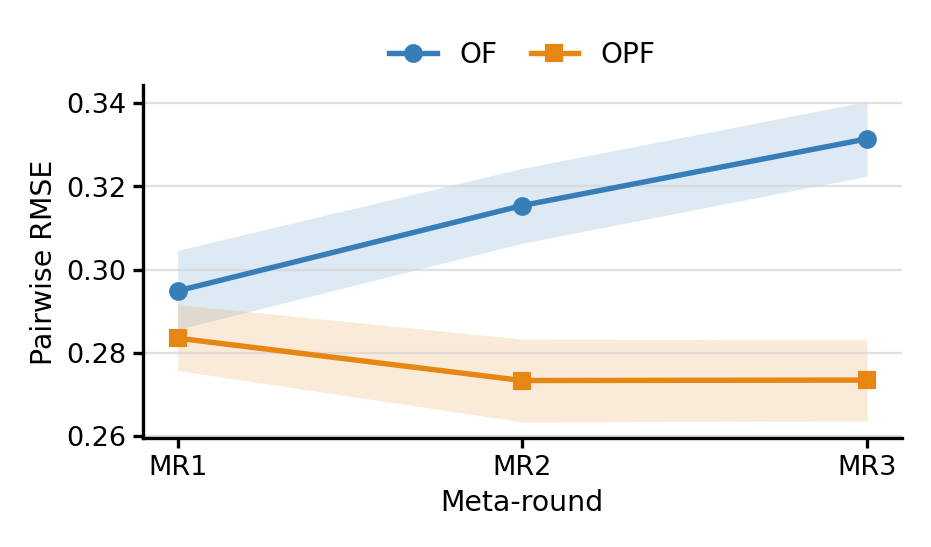
\includegraphics[width=0.90\linewidth]{policy_convergence.png}
    \caption{Behavioral convergence across meta-rounds. Distance is the
    within-experiment mean pairwise RMSE between normalized bids on 144
    controlled states; lower values indicate more similar behavior. Shaded
    regions are 95\% matched experiment-cluster bootstrap intervals.}
    \label{fig:policy-convergence}
\end{figure}

Figure~\ref{fig:policy-convergence} shows that the two feedback conditions
produce qualitatively different policy dynamics. Under OF, behavioral
distance increases across revisions; under OPF, it decreases after the first
policy exposure and then remains stable. The baseline-adjusted MR1--MR3
contrast confirms this divergence. A normalized-AST analysis yields the same
qualitative pattern and is reported in the supplementary appendix.

Access to decision rules therefore changes not only outcomes but also the
policy population, moving agents toward a more shared bidding repertoire
despite asymmetric roles. Descriptive outcome dispersion moves in the same
direction and is reported in the appendix. We interpret BPD as evidence of
policy-population adaptation: it establishes behavioral alignment without
requiring a claim about direct copying from any particular opponent.

\subsection{Failure Mechanisms}

We complement multi-seed outcome evaluation with a mechanism analysis of the
original policy-generation trajectories. Among 3,600 valid agent-rounds,
1,444 end in death, and every case receives valid outputs from both judges.
This analysis conditions on the shared experienced trajectory and asks which
policy mechanisms recur across failed executions.

The attribution stage prevents every death from being forced into a policy
failure. Averaging the two judges' votes, 67.9\% of deaths are
policy-dominant and 22.4\% involve policy interacting with adverse context;
the remainder have no clear policy failure or insufficient evidence.
Figure~\ref{fig:failure-modes} reports primary diagnoses across all death
cases rather than normalizing only the policy-attributable subset. Role
exposure is shown separately because it describes initial context rather
than a policy mechanism.

\begin{figure}[t]
    \centering
    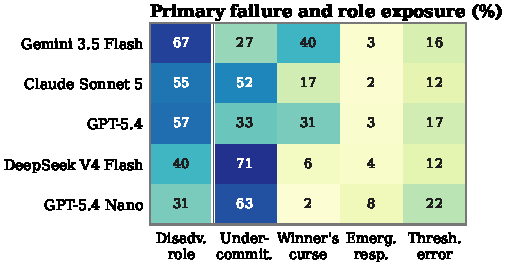
\includegraphics[width=0.92\linewidth]{failure_analysis_figures/primary_failure_with_role_heatmap.pdf}
    \caption{Disadvantaged-role exposure and primary failure diagnoses among
    deaths. Each cell is a percentage of that model's death cases.
    Disadvantaged-role exposure is rule-based; for each policy mechanism,
    each judge contributes half a vote when selecting it as primary. Role
    exposure can overlap with a diagnosis, and omitted diagnoses mean that
    displayed rows need not sum to 100\%.}
    \label{fig:failure-modes}
\end{figure}

Figure~\ref{fig:failure-modes} reveals different failure signatures despite
the shared game interface. Deaths of Gemini 3.5 Flash, Claude Sonnet 5, and
GPT-5.4 occur disproportionately often in the disadvantaged role, whereas
the weaker backends fail across a wider range of roles. DeepSeek V4 Flash
and GPT-5.4 Nano are dominated by fatal undercommitment, and Nano also shows
the highest rate of competitive-threshold miscalibration. Gemini instead has
a winner's-curse-heavy primary profile, consistent with costly earlier wins
weakening later survival; this operationalizes the overpayment mechanism
observed in the original WAC study~\cite{mao2025alympics}. GPT-5.4 lies
between these patterns, with diagnoses split more evenly between
undercommitment and winner's-curse overpayment.

Attribution-status agreement is 81.2\% ($\kappa=0.610$), while exact
agreement on the primary diagnosis is 61.6\% ($\kappa=0.436$). Thus, the
judges agree more strongly on whether policy failure contributed than on its
fine-grained mechanism. We use their averaged primary votes to compare
model-level failure signatures, while retaining simulator events as the
objective evidence for each case.

\section{Limitations}

WACBench provides controlled policy evaluation within one repeated
resource-allocation setting, so its conclusions concern the tested backends,
opponent pools, and scarcity regime. Policies revise from one shared
experienced trajectory, while five-seed replay measures transfer to four
held-out supply sequences. OF and OPF use independent MR1 generations;
matched baseline changes and common replays provide the policy-access
comparison. The fixed heuristic is an interpretable reference rather than an
optimal bound. Behavioral convergence is measured on a controlled state
grid, and post-hoc failure labels complement rather than replace deterministic
outcomes. Extending WACBench across environments, experienced trajectories,
opponent cohorts, and reference families is a natural direction for broader
evaluation.

\section{Conclusion}

We introduced WACBench, a code-mediated benchmark for evaluating strategic
adaptation in a repeated, asymmetric resource competition environment.
Treating executable policies as the unit of decision making makes the
implemented decision rule persistent, permits exact replay, and exposes the
links among a model's rationale, policy, actions, and realized trajectory.
Frozen-opponent replays show that both feedback conditions yield effective
first revisions. The three-round trajectories reveal the later divergence:
OF largely plateaus, whereas OPF sustains later WACScore gains and moves aggregate
policies from parity with a fixed heuristic to a positive survival-duration
advantage.

Controlled probes show that OPF also makes policies more similar in bidding
behavior and program structure, demonstrating that policy access reshapes the
evolving strategy population as well as survival outcomes. The failure
heatmap further identifies distinct undercommitment- and overpayment-heavy
signatures across model backends. Together, these results establish
executable-policy evaluation, controlled replay, calibrated references, and
auditable failure mechanisms as a practical framework for studying strategic
LLM adaptation.

% Uncomment and replace with your bibliography file when ready.
\bibliography{aaai2027}

\end{document}
